% !TEX root =  master.tex
\section{Konzept}
\label{sec:konzept}
\authorsection{\authorSG}
In diesem Projekt soll die Drei-Schichten-Architektur eingesetzt werden.
Sie dient dazu, die einzelnen Schichten (Datenhaltung, Fachkonzept und Benutzeroberfläche) zu separieren, sodass in zukünftigen Schritten ein Austausch der genutzten Benutzeroberfläche oder Datenbank möglich ist. 

Wie zuvor in Kapitel \vref{sec:technologien} beschrieben, finden in diesem Projekt \acs{REST}ful Webservices Anwendung.
Da Webservices in der Realität u.a. aus Performance-Gründen auf unterschiedlichen Servern ausgeführt werden, wurde dies hier ebenfalls umgesetzt.
Zum Einsatz kommt eine System- und Data-Webservice.
Wie in Abbildung \vref{fig:konzept_backend} dargestellt ist, greift die Benutzeroberfläche niemals direkt auf die Datenhaltungsschicht zu.
Dies wird realisiert, indem das Front-End auf die bereitgestellten Webservices von System in der Fachkonzeptschicht zugreift. 
Diese wiederum greifen dann auf die Webservices der Datenhaltungsschicht zu.

\begin{figure}[ht]
	\centering
	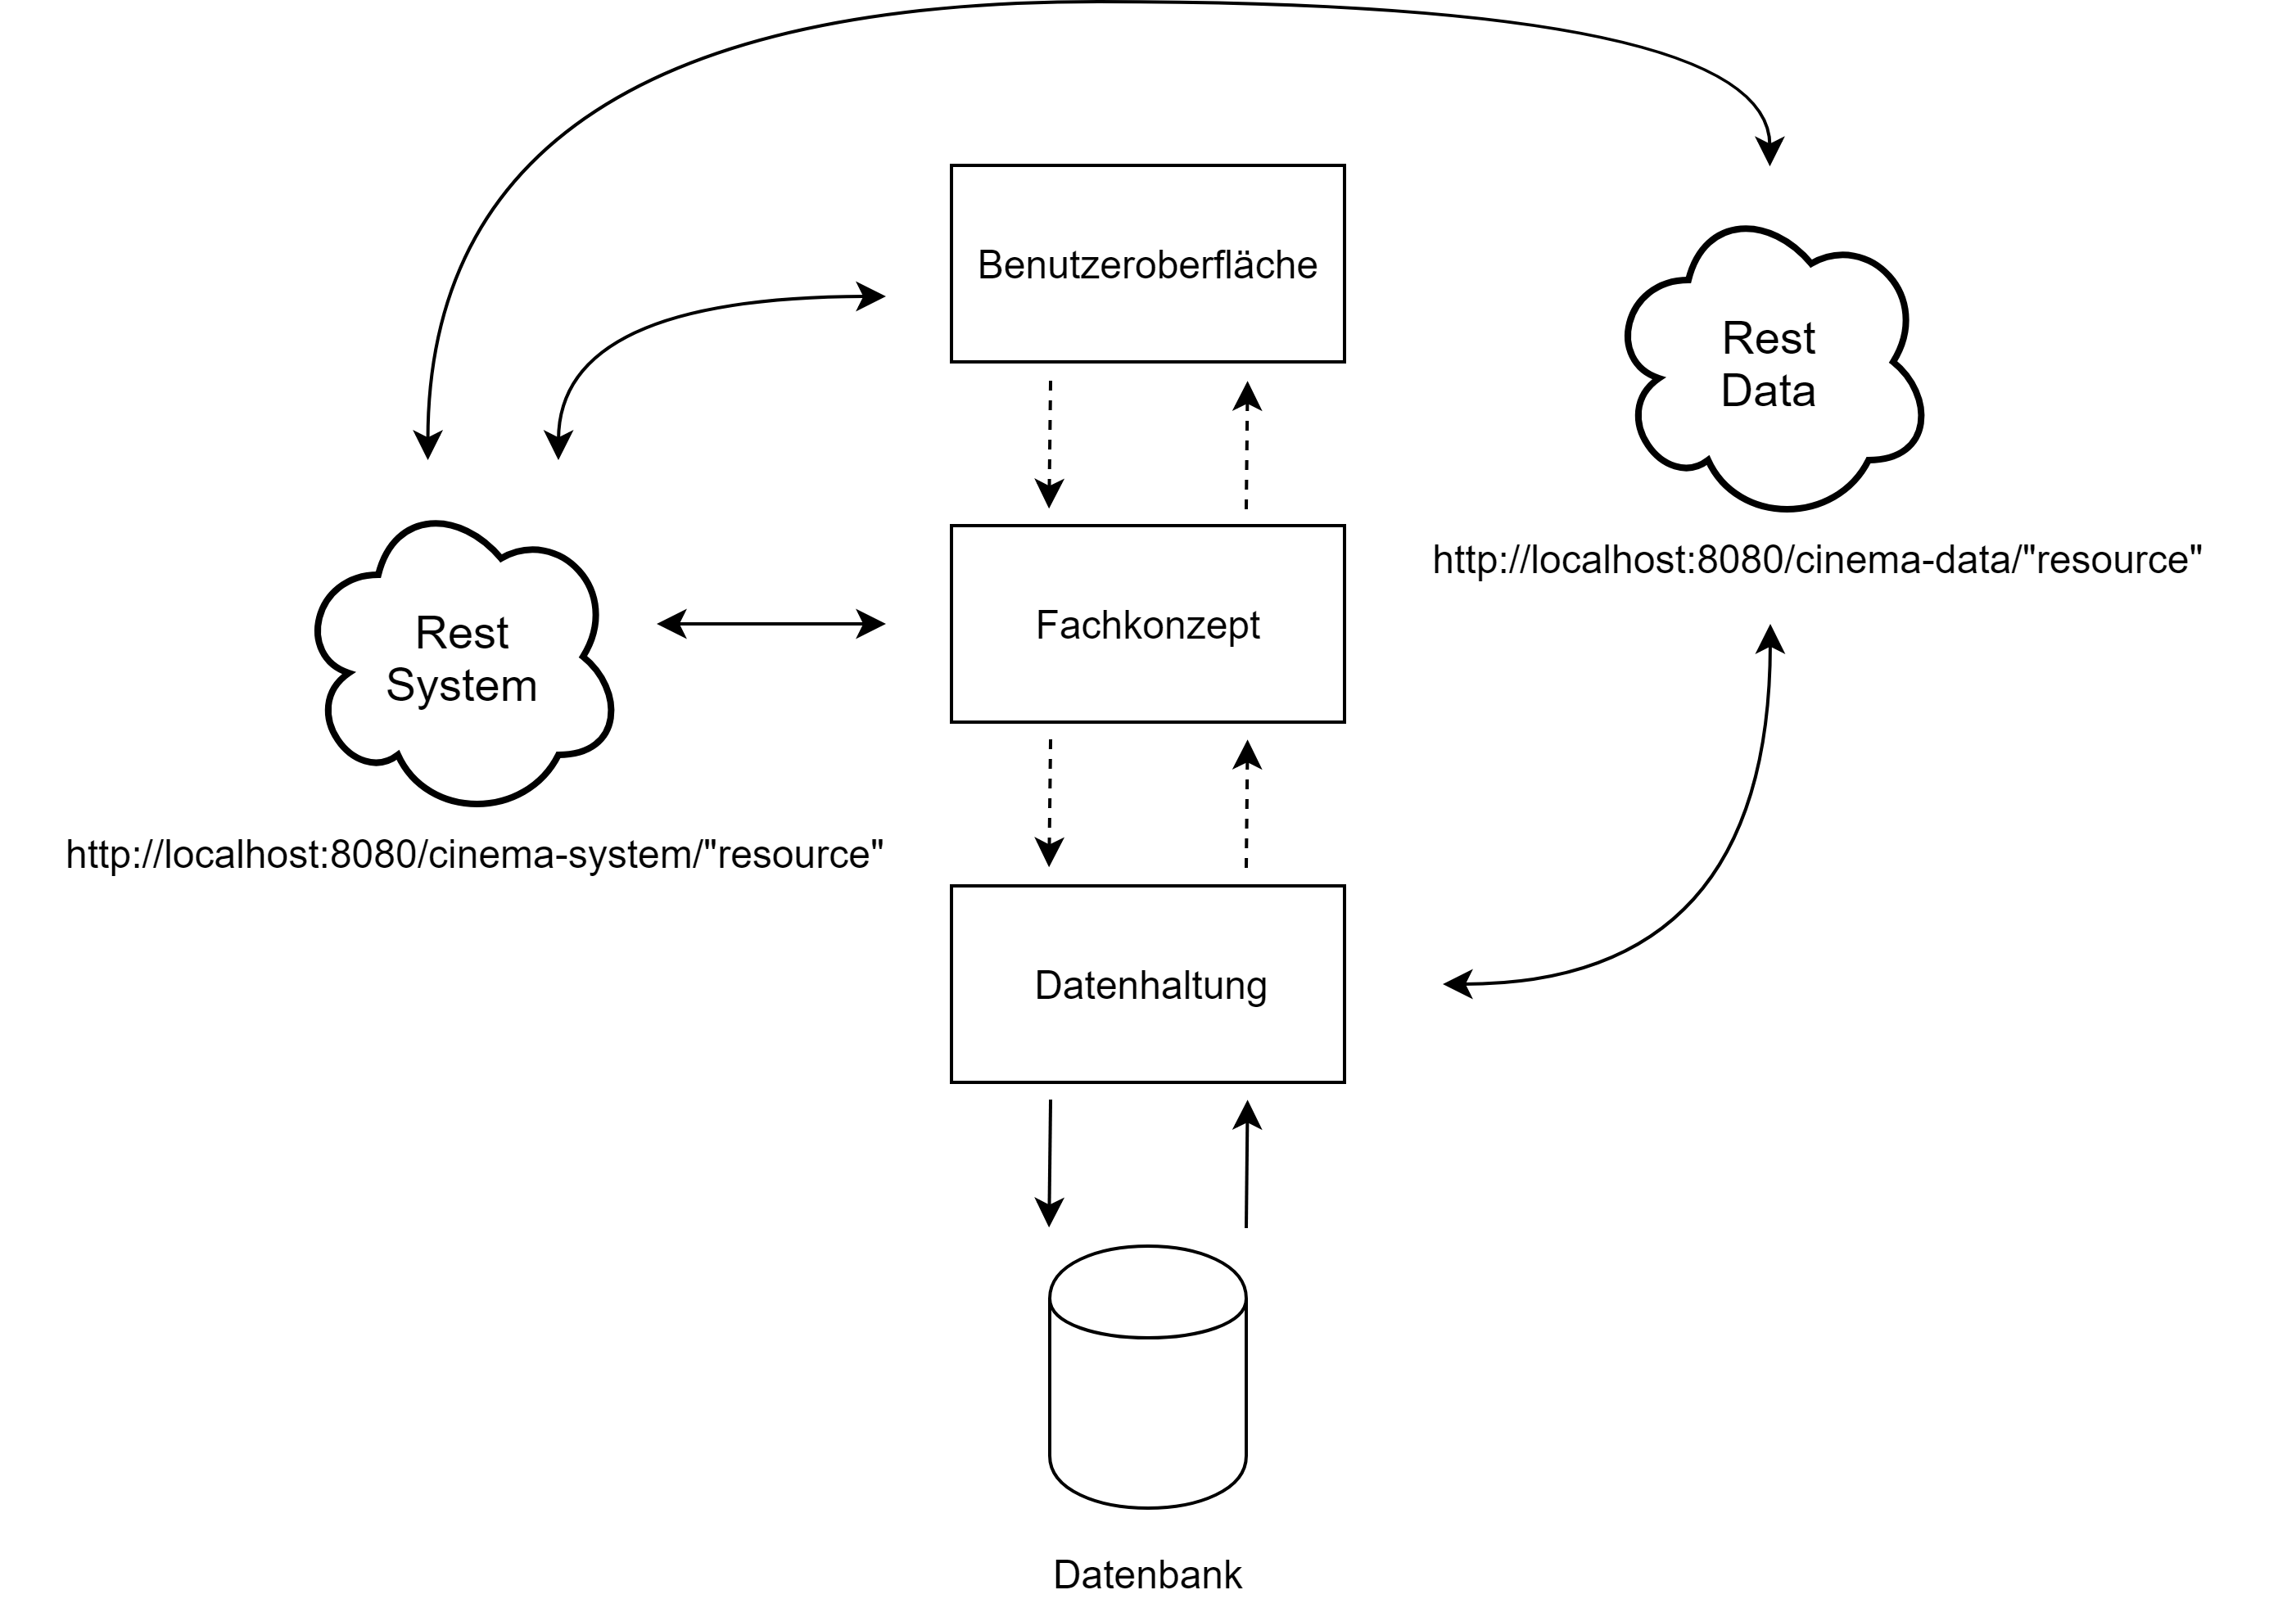
\includegraphics[width=0.7\textwidth]{img/backend/rest}
	\captionsetup{format=hang}
	\caption{Konzept des Back-Ends}
	\small Quelle: eigene Darstellung mittels \url{https://draw.io/}
	\label{fig:konzept_backend}
	\end{figure}

Für dieses Projekt werden drei Hauptklassen in Java verwendet: \textit{Shared}, \textit{System} und \textit{Data}. 
In der Klasse \textit{Shared} befinden sich alle gemeinsam genutzten Klassen wie z.B. u.a. die verwendeten \acp{DTO}, Konvertierungs-Methoden, ausgelagerten Überprüfungen und der \acs{JSON}-Converter, der das \acs{DTO} in ein \acs{JSON} umwandelt. 

Die System-Ressource stellt dem Front-End mehrere \acs{REST}-Schnittstellen zur Verfügung.
Nachdem die Ressource über eine \acs{URI} \url{http://localhost:8080/cinema-system/show/1} aufgerufen wurde, ruft diese z.B. die Methode \jinline |getMovieById| in ihrem eigenen Service auf.
Diese ruft den Webservice \url{http://localhost:8080/cinema-data/show/1} in der Data-Ressource auf, welche die gewünschten Daten über die dort gleichnamige implementierte Methode im eigenen \textit{ShowService} aufruft. Diese Methode ruft anschließend das Show-\acs{DAO} auf, welches die Datensätze in der Datenbank anfragt. 
Die erhaltenen Datensätze werden daraufhin in ein Show-\acf{DTO} umgewandelt und an die System-Ressource zurückgegeben.
Eine Erläuterung warum dies notwendig ist, wird in Kapitel \vref{sec:dto} näher beschrieben. \\
Jede Ressource hat wiederum mehrere Services implementiert, die die gewünschten Anfragen bearbeitet und konsolidieren.

Die Erläuterung wie dies seitens des Front-Ends umgesetzt ist, wird in Kapitel \vref{sec:anbindung_backend} näher erläutert.
 
%Möchte man z.B. alle Daten einer Vorstellung haben, so ruft das Front-End die Ressource mit der \acs{URI} \url{http://localhost:8080/cinema-system/show/1} auf.

Die aktuell verwendeten Ressourcen in diesem Projekt sind:
\begin{itemize}
	\item show $\rightarrow$ hier können alle Informationen über die Vorstellungen abgerufen werden
	\item reservation $\rightarrow$ alles was mit der Reservierung bzw. Blocken in Abhängigkeit steht 
	\item movie $\rightarrow$ hier können alle Informationen über eine Film abgerufen werden
	\item employee $\rightarrow$ hier können alle Informationen über die Mitarbeiter des Kinos abgerufen werden
\end{itemize} 

Diese haben jeweils einen eigenen Service, der für die Kommunikation zwischen den Ressourcen, den Webservices und der Datenbank verantwortlich ist. 